\subsection{Rectifiers, Regulators, etc.}
\label{subsec:rect-reg}

\subsubsection*{Rectifiers: Turning AC into DC}
Let's start with rectifiers, the power behind the throne of the electronics world. A rectifier is a device that converts alternating current (AC) into direct current (DC). Think of it as a traffic cop for electrons, only letting them flow in one direction. This is crucial because many electronic devices, like your smartphone or laptop, need DC to function properly. The rectifier achieves this by using diodes, which act like one-way valves for electrical current. 

For example, in a simple half-wave rectifier, only the positive half of the AC waveform is allowed through, while the negative half is blocked. A full-wave rectifier, on the other hand, flips the negative half of the waveform to make it positive, resulting in a smoother DC output. You can see this process illustrated in Figure~\ref{fig:rectifier}.

\begin{figure}[h]
    \centering
    \footnotesize
    \begin{minipage}{0.4\textwidth}
        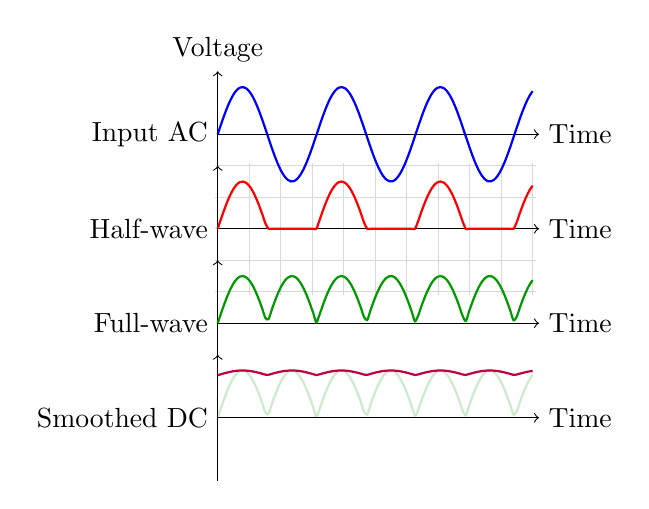
\begin{tikzpicture}[scale=0.4]
            % Grid for all plots
            \draw[gray!30, step=1] (-0.1,-2.1) grid (10.1,2.1);
            
            % Input AC Signal
            \begin{scope}[yshift=3cm]
                \draw[->] (0,0) -- (10.2,0) node[right] {Time};
                \draw[->] (0,-2) -- (0,2) node[above] {Voltage};
                \draw[blue, thick, smooth] plot[domain=0:10,samples=100] 
                    (\x,{1.5*sin(2*\x r)});
                \node[left] at (0,0) {Input AC};
            \end{scope}
            
            % Half-wave rectified
            \begin{scope}[yshift=0cm]
                \draw[->] (0,0) -- (10.2,0) node[right] {Time};
                \draw[->] (0,-2) -- (0,2) node[above] {};
                \draw[red, thick, smooth] plot[domain=0:10,samples=100] 
                    (\x,{max(0,1.5*sin(2*\x r))});
                \node[left] at (0,0) {Half-wave};
            \end{scope}
            
            % Full-wave rectified
            \begin{scope}[yshift=-3cm]
                \draw[->] (0,0) -- (10.2,0) node[right] {Time};
                \draw[->] (0,-2) -- (0,2) node[above] {};
                \draw[green!60!black, thick, smooth] plot[domain=0:10,samples=100] 
                    (\x,{abs(1.5*sin(2*\x r))});
                \node[left] at (0,0) {Full-wave};
            \end{scope}
            
            % Smoothed DC (with capacitor)
            \begin{scope}[yshift=-6cm]
                \draw[->] (0,0) -- (10.2,0) node[right] {Time};
                \draw[->] (0,-2) -- (0,2) node[above] {};
                % Base full-wave rectified
                \draw[green!60!black, thick, smooth, opacity=0.2] plot[domain=0:10,samples=100] 
                    (\x,{abs(1.5*sin(2*\x r))});
                % Smoothed output
                \draw[purple, thick, smooth] plot[domain=0:10,samples=100] 
                    (\x,{1.35+0.15*abs(sin(2*\x r))});
                \node[left] at (0,0) {Smoothed DC};
            \end{scope}
        \end{tikzpicture}
        \caption*{(a) Waveforms showing AC to DC conversion process}
    \end{minipage}%
    \hfill%
    \begin{minipage}{0.4\textwidth}
        \begin{circuitikz}[scale=0.4],american]
            % AC source
            \draw (0,5) to[sinusoidal voltage source, l_=AC] (0,-5);
        
            \draw (0,-5) -- (6,-5) -- (6, -4);
            \draw (0,5) -- (6,5) -- (6,4);
            \draw[->] (2,0) -- (1,0) -- (1,-6) --(12,-6)node[right]{$-$};
            \draw[->] (10,0) -- (12,0)node[right]{$+$};
            
            \draw (2,0)  to[D, -] (6,-4);
            \draw (6,-4)  to[D, -] (10,0);
            \draw (2,0)   to[D, -] (6,4);
            \draw (6,4)  to[D, -] (10,0);
             \draw[<->,dashed] (12,-6) -- (12,0) node[midway,above] {DC}; 
        \end{circuitikz}
        
        \caption*{(b) Four-diode bridge rectifier circuit}
    \end{minipage}
    \caption{AC to DC conversion using rectifiers. (a) Shows the progression from AC input to smoothed DC output: original AC signal, half-wave rectification, full-wave rectification, and smoothed DC after filtering. (b) Shows a typical bridge rectifier circuit that performs full-wave rectification using four diodes.}
    \label{fig:rectifier}
\end{figure}
    
\begin{table}[h]
    \centering
    \caption{Comparison of rectifier types.}
    \label{tab:rectifiers}
    \begin{tabular}{|l|l|l|}
    \hline
    \textbf{Type} & \textbf{Efficiency} & \textbf{Output} \\
    \hline
    Half-wave & Low & Pulsating DC \\
    Full-wave & Higher & Smoother DC \\
    Bridge & Highest & Smoother DC \\
    \hline
    \end{tabular}
\end{table}
    



\subsubsection*{Relays: The Electrically-Controlled Switch}
Next up, we have relays. A relay is essentially an electrically-controlled switch. When you send a small current through the relay's coil, it creates a magnetic field that pulls a switch to connect or disconnect a larger current. This is super handy when you want to control a high-power circuit with a low-power signal, like turning on a motor with a tiny button. 

% add a figure of a relay
\begin{figure}[h]
    \centering
    \begin{minipage}{0.24\textwidth}
        \includegraphics[width=\textwidth]{tech/images/relay.jpg}
        \caption*{(a) Relay}
    \end{minipage}%
    \hfill%
    \begin{minipage}{0.24\textwidth}
        \includegraphics[width=\textwidth]{tech/images/transformer.jpg}
        \caption*{(b) Transformer}
    \end{minipage}%
    \hfill%
    \begin{minipage}{0.24\textwidth}
        \centering
        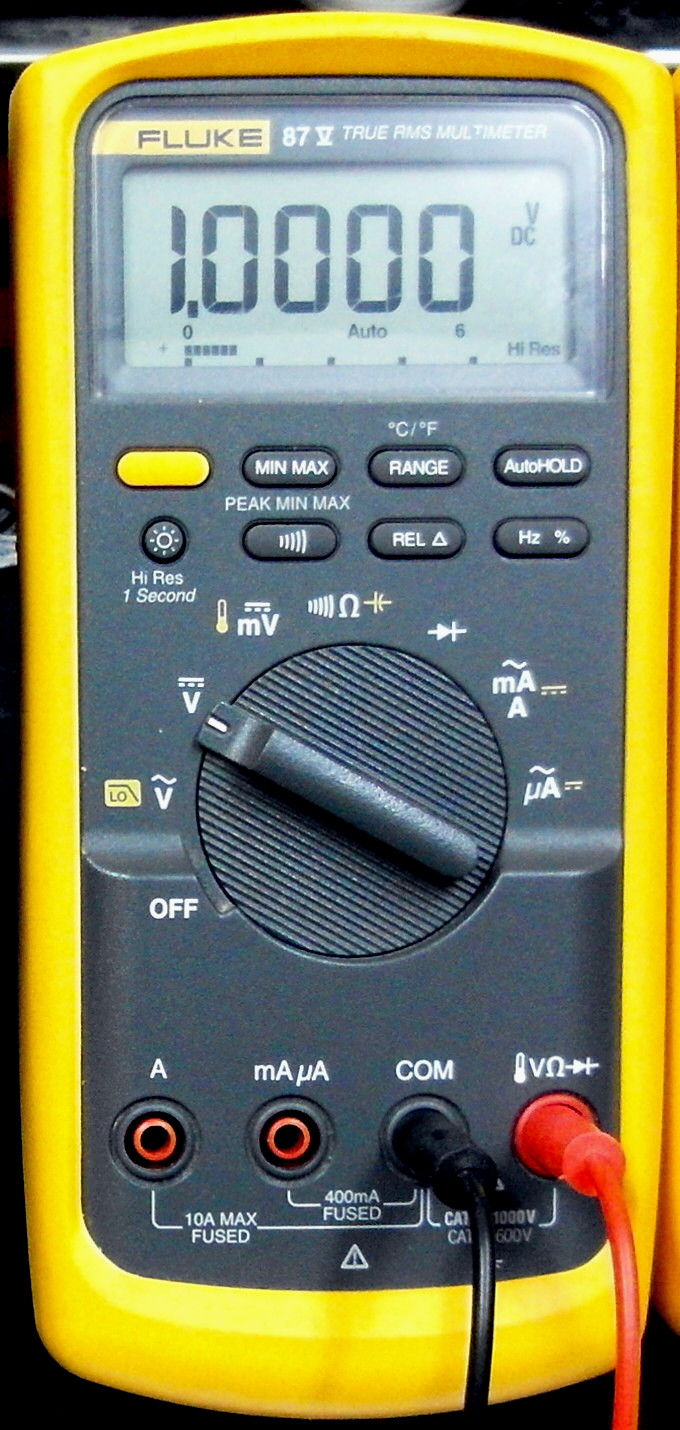
\includegraphics[width=0.5\textwidth]{tech/images/multimeter.jpg}
        \caption*{(c) Multimeter}
    \end{minipage}%
    \hfill%
    \begin{minipage}{0.24\textwidth}
        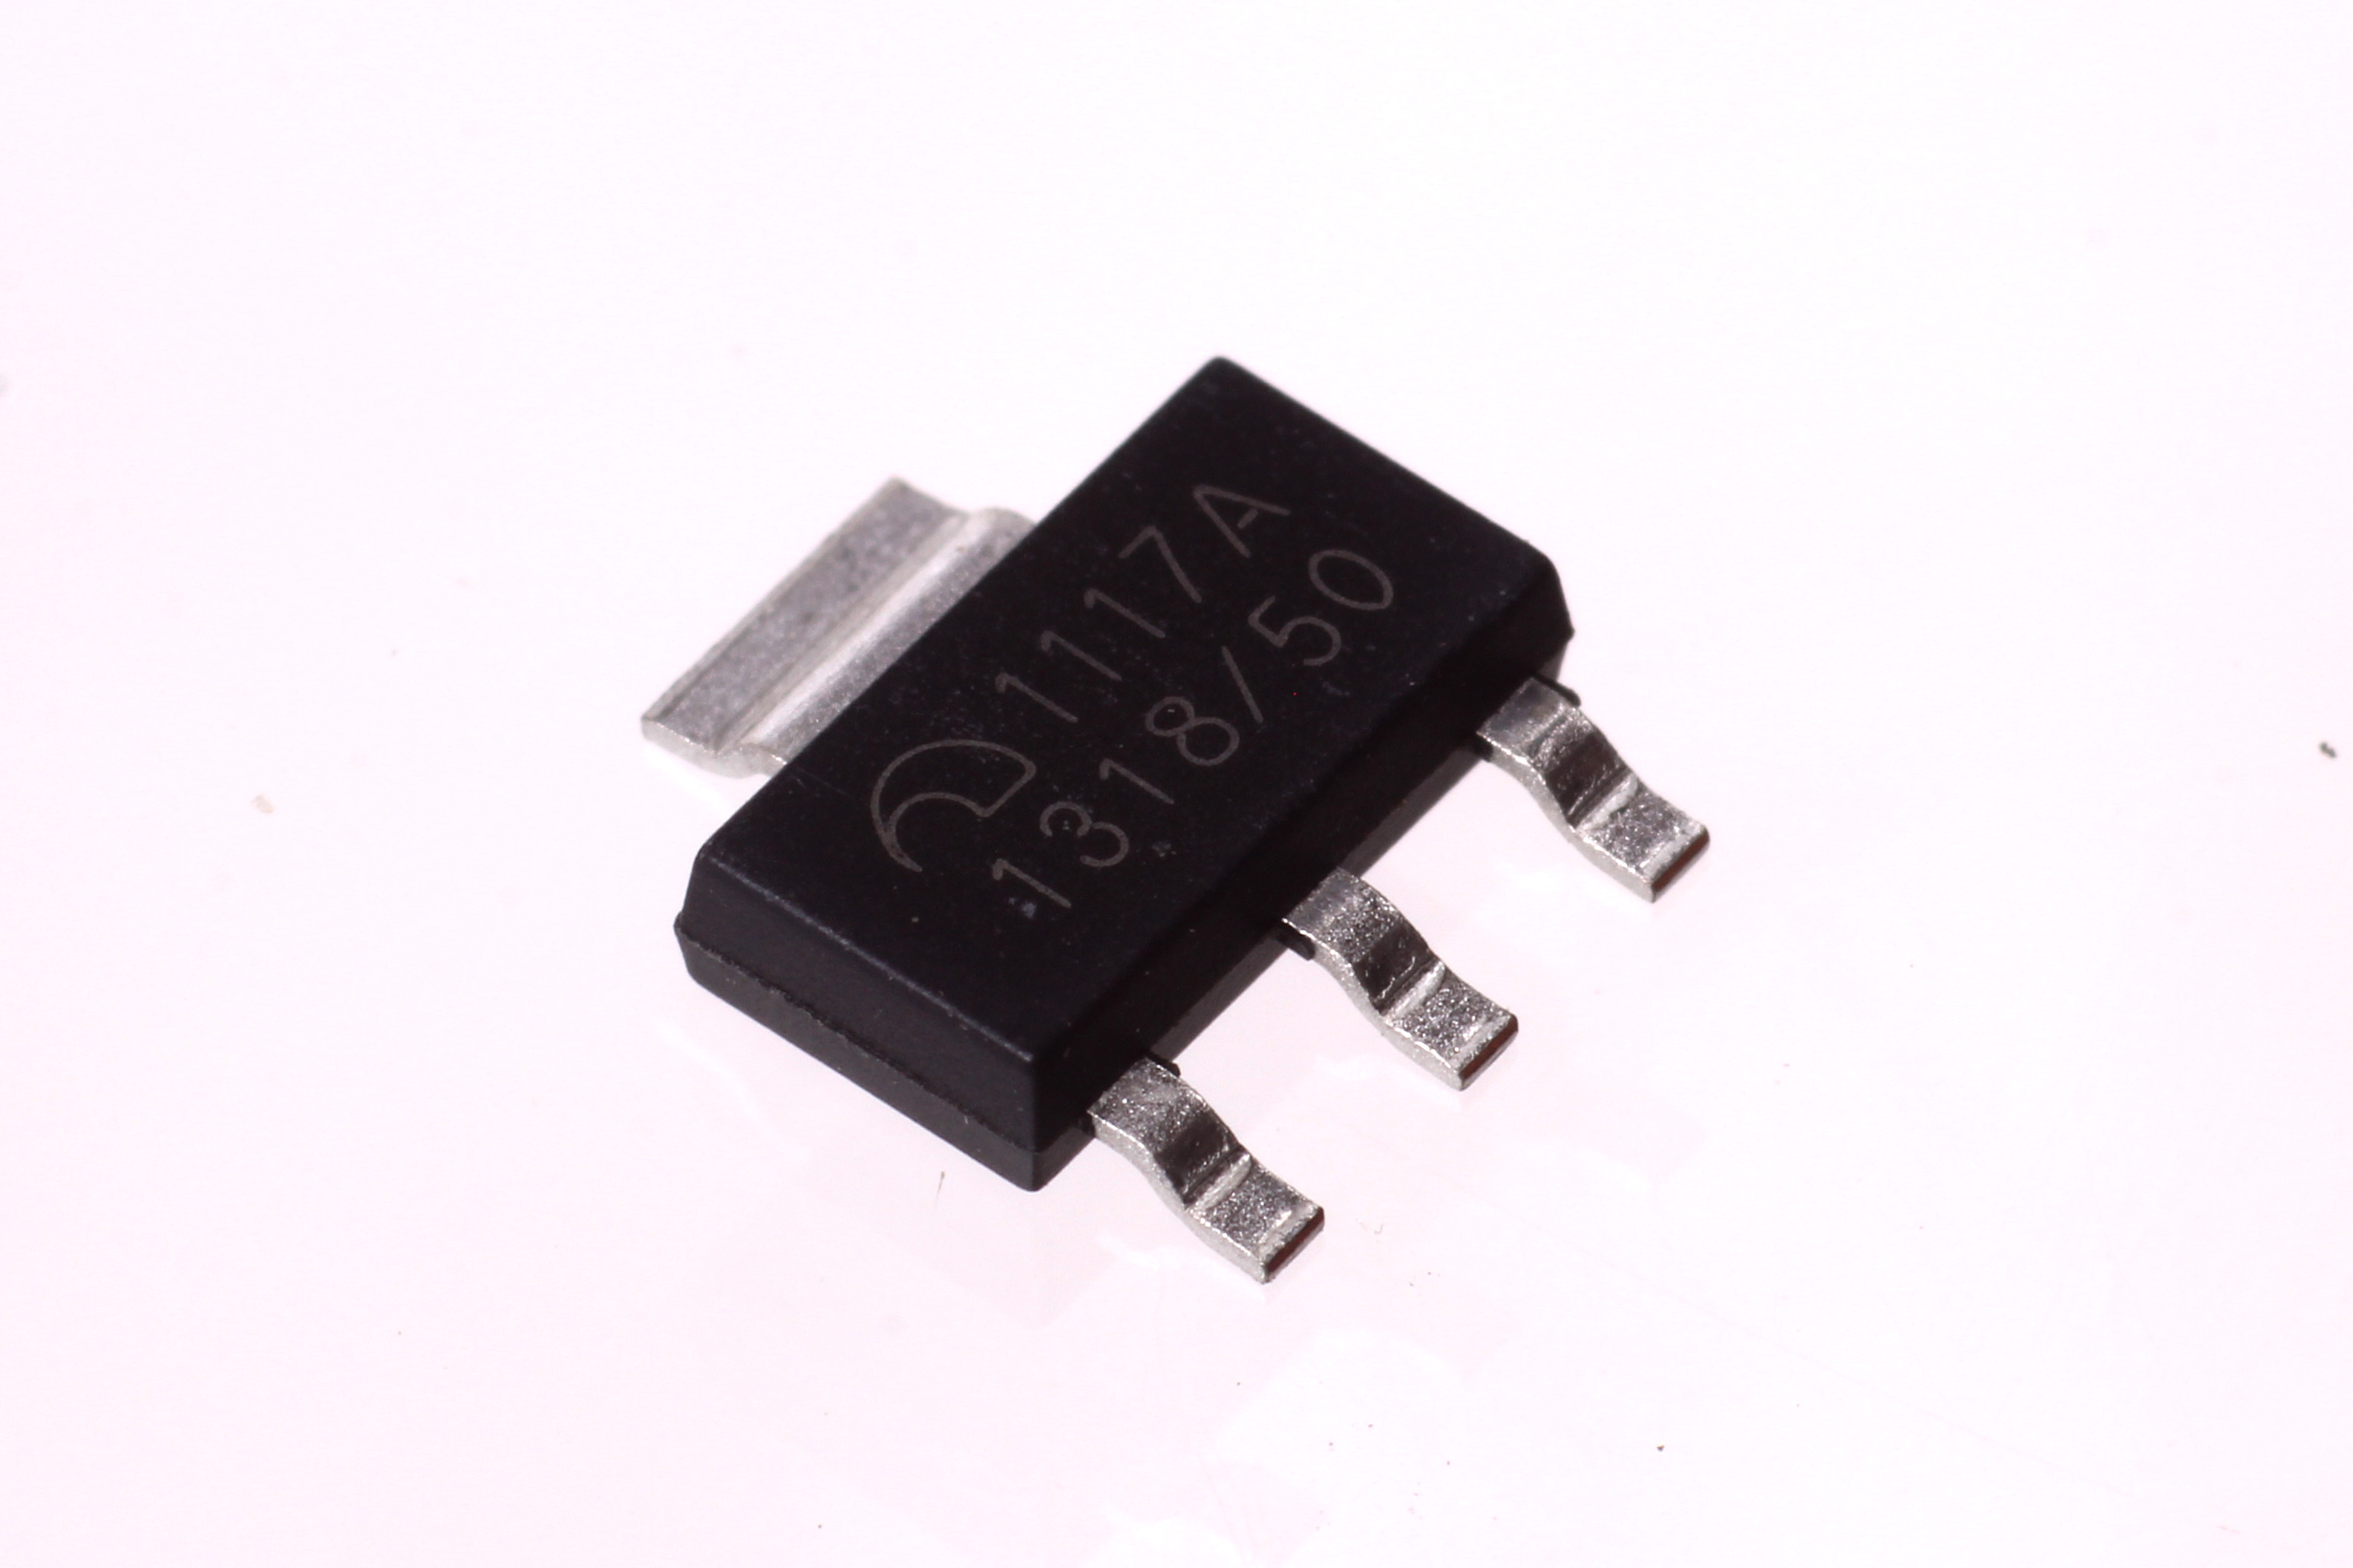
\includegraphics[width=\textwidth]{tech/images/regulator.jpg}
        \caption*{(d) Voltage Regulator}
    \end{minipage}
    \caption{Common electronic components: (a) A relay for switching high-power circuits with low-power signals, (b) A transformer for changing AC voltage levels, (c) A multimeter for measuring electrical quantities, and (d) A voltage regulator for maintaining constant output voltage.}
    \label{fig:electronic-components}
\end{figure}


\subsubsection*{Shielded Wire: Keeping Signals Clean}
Ever wonder why some wires are wrapped in a metallic braid? That's shielded wire, and its job is to prevent unwanted signal coupling. In other words, it keeps your signals from getting mixed up with other signals nearby. This is especially important in radio circuits, where even a tiny bit of interference can mess things up. 

\subsubsection*{Meters: The Numeric Display of Electrical Quantities}
Meters are the gadgets that give you a numeric readout of electrical quantities like voltage, current, or resistance. They’re like the speedometer in your car, but for electricity. Whether it's an analog needle or a digital display, meters help you keep track of what's going on in your circuit.

\subsubsection*{Regulators: Keeping Voltage in Check}
A voltage regulator is like a thermostat for your power supply. It maintains a constant output voltage even when the input voltage or load current changes. Inside a typical linear regulator, a feedback circuit continuously monitors the output voltage and adjusts a control element (usually a transistor) to maintain the desired voltage level. For example, if the output voltage starts to drop due to increased load, the regulator compensates by allowing more current to flow through. Common regulators like the 7805 can take a varying input of 7-35V and provide a steady 5V output, perfect for powering digital circuits.

\subsubsection*{Transformers: Changing AC Voltage Levels}
Transformers are the workhorses of AC circuits. They can step up (increase) or step down (decrease) AC voltage levels. This is done using two coils of wire wrapped around a common core. When AC flows through the primary coil, it creates a magnetic field that induces a voltage in the secondary coil. The ratio of the number of turns in the coils determines the voltage change. For example, if you need to step down 120 V AC to 12 V AC, a transformer is your go-to device.

\subsubsection*{LEDs: The Visual Indicators}
Finally, let's talk about LEDs, or Light Emitting Diodes. These little guys are everywhere, from your TV remote to the indicator lights on your stereo. LEDs are great because they’re energy-efficient, long-lasting, and come in a variety of colors. They’re the perfect way to give you a visual cue about what’s happening in your circuit.



% \begin{figure}[h]
% \centering
% % \includegraphics{relay.svg} % Placeholder for the relay schematic
% \caption{Relay circuit schematic.}
% \label{fig:relay}
% % Prompt: Schematic of a relay circuit.
% \end{figure}

% \begin{figure}[h]
% \centering
% % \includegraphics{shielded-wire.svg} % Placeholder for the shielded wire illustration
% \caption{Shielded wire preventing signal interference.}
% \label{fig:shielded-wire}
% % Prompt: Illustration of shielded wire preventing signal interference.
% \end{figure}

\subsubsection*{Questions}

\begin{tcolorbox}[colback=gray!10!white,colframe=black!75!black,title={T6D01}]
Which of the following devices or circuits changes an alternating current into a varying direct current signal?
\begin{enumerate}[label=\Alph*),noitemsep]
    \item Transformer
    \item \textbf{Rectifier}
    \item Amplifier
    \item Reflector
\end{enumerate}
\end{tcolorbox}
A rectifier is specifically designed to convert AC to DC. Transformers change voltage levels, amplifiers increase signal strength, and reflectors are used in antennas, not for current conversion.

\begin{tcolorbox}[colback=gray!10!white,colframe=black!75!black,title={T6D02}]
What is a relay?
\begin{enumerate}[label=\Alph*),noitemsep]
    \item \textbf{An electrically-controlled switch}
    \item A current controlled amplifier
    \item An inverting amplifier
    \item A pass transistor
\end{enumerate}
\end{tcolorbox}
A relay uses a small electrical current to control a larger one, acting as a switch. The other options describe different types of amplifiers or transistors, not relays.

\begin{tcolorbox}[colback=gray!10!white,colframe=black!75!black,title={T6D03}]
Which of the following is a reason to use shielded wire?
\begin{enumerate}[label=\Alph*),noitemsep]
    \item To decrease the resistance of DC power connections
    \item To increase the current carrying capability of the wire
    \item \textbf{To prevent coupling of unwanted signals to or from the wire}
    \item To couple the wire to other signals
\end{enumerate}
\end{tcolorbox}
Shielded wire is used to prevent interference, not to change resistance or current capacity. Coupling signals is the opposite of what shielded wire is designed to do.

\begin{tcolorbox}[colback=gray!10!white,colframe=black!75!black,title={T6D04}]
Which of the following displays an electrical quantity as a numeric value?
\begin{enumerate}[label=\Alph*),noitemsep]
    \item Potentiometer
    \item Transistor
    \item \textbf{Meter}
    \item Relay
\end{enumerate}
\end{tcolorbox}
Meters are designed to display electrical quantities like voltage, current, or resistance numerically. The other components do not have this function.

\begin{tcolorbox}[colback=gray!10!white,colframe=black!75!black,title={T6D05}]
What type of circuit controls the amount of voltage from a power supply?
\begin{enumerate}[label=\Alph*),noitemsep]
    \item \textbf{Regulator}
    \item Oscillator
    \item Filter
    \item Phase inverter
\end{enumerate}
\end{tcolorbox}
A regulator maintains a constant voltage output, regardless of changes in input voltage or load. Oscillators generate signals, filters remove unwanted frequencies, and phase inverters change the phase of a signal.

\begin{tcolorbox}[colback=gray!10!white,colframe=black!75!black,title={T6D06}]
What component changes 120 V AC power to a lower AC voltage for other uses?
\begin{enumerate}[label=\Alph*),noitemsep]
    \item Variable capacitor
    \item \textbf{Transformer}
    \item Transistor
    \item Diode
\end{enumerate}
\end{tcolorbox}
Transformers are specifically designed to change AC voltage levels. Capacitors, transistors, and diodes do not perform this function.

\begin{tcolorbox}[colback=gray!10!white,colframe=black!75!black,title={T6D07}]
Which of the following is commonly used as a visual indicator?
\begin{enumerate}[label=\Alph*),noitemsep]
    \item \textbf{LED}
    \item FET
    \item Zener diode
    \item Bipolar transistor
\end{enumerate}
\end{tcolorbox}
LEDs are widely used as visual indicators due to their low power consumption and bright light output. The other components are not typically used for this purpose.
